\documentclass[10pt,a4paper]{article}

% ---------- Packages ----------
\usepackage[a4paper,margin=2cm,top=1.8cm,bottom=2cm]{geometry}
\usepackage[T1]{fontenc}
\usepackage[utf8]{inputenc}
\usepackage{lmodern}
\usepackage[scaled=0.95]{helvet}
\renewcommand{\familydefault}{\sfdefault}
\usepackage{microtype}
\usepackage{xcolor}
\usepackage{tabularx}
\usepackage{booktabs}
\usepackage{array}
\usepackage{enumitem}
\usepackage{titlesec}
\usepackage{fancyhdr}
\usepackage{tikz}
\usetikzlibrary{arrows.meta,fit,backgrounds}
\usepackage[hidelinks]{hyperref}

% ---------- Colours (one per block category, used in the diagrams) ----------
\definecolor{ink}{HTML}{1B2033}
\definecolor{muted}{HTML}{5D6479}
\definecolor{accent}{HTML}{1F3FBF}
\definecolor{cTrig}{HTML}{DCE6FB}   % triggers / replies
\definecolor{cLogic}{HTML}{FCEFC7}  % Switch / If / Set
\definecolor{cCode}{HTML}{E6E8EE}   % Code nodes
\definecolor{cApi}{HTML}{EADDFB}    % external APIs
\definecolor{cAI}{HTML}{FDE0CC}     % AI nodes
\definecolor{cDB}{HTML}{D7F0DF}     % database
\definecolor{cSub}{HTML}{CDEFEF}    % sub-workflow
\definecolor{cErr}{HTML}{FBDADA}    % error handling

\color{ink}
\setlength{\parindent}{0pt}
\setlength{\parskip}{5pt}
\setlist{itemsep=2pt,topsep=3pt,leftmargin=1.4em}

\titleformat{\section}{\large\bfseries\color{ink}}{\color{accent}\thesection}{0.6em}{}
\titlespacing*{\section}{0pt}{12pt}{4pt}
\titleformat{\subsection}{\normalsize\bfseries\color{ink}}{}{0em}{}
\titlespacing*{\subsection}{0pt}{8pt}{2pt}

\pagestyle{fancy}
\fancyhf{}
\renewcommand{\headrulewidth}{0pt}
\fancyfoot[L]{\footnotesize\color{muted}Deadline Coach \textperiodcentered{} Saty Viard Laroque}
\fancyfoot[R]{\footnotesize\color{muted}\thepage}

\newcommand{\cmd}[1]{\texttt{\small #1}}
\newcommand{\legendtag}[2]{\colorbox{#1}{\strut\footnotesize #2}}

% ---------- TikZ styles ----------
\tikzset{
  blk/.style={draw=ink!55, rounded corners=2pt, align=center, font=\scriptsize,
              minimum height=8.5mm, inner sep=2pt, text width=17mm,
              execute at begin node={\hyphenpenalty=10000\exhyphenpenalty=10000}},
  trig/.style={blk, fill=cTrig},
  logic/.style={blk, fill=cLogic},
  code/.style={blk, fill=cCode},
  api/.style={blk, fill=cApi},
  ai/.style={blk, fill=cAI},
  db/.style={blk, fill=cDB},
  sub/.style={blk, fill=cSub},
  err/.style={blk, fill=cErr},
  ref/.style={blk, fill=white, dashed},
  arr/.style={-{Stealth[length=1.8mm]}, draw=ink!70, semithick},
  lbl/.style={font=\tiny\color{muted}, fill=white, inner sep=1pt},
  frame/.style={draw=ink!25, dashed, rounded corners=4pt, inner sep=5pt},
  ftitle/.style={font=\footnotesize\bfseries\color{ink}, anchor=south west}
}

\begin{document}

% ================= Title block =================
{\footnotesize\color{muted}\textsc{No-Code Software Development \textperiodcentered{} Project Report}}\par\vspace{2pt}
{\LARGE\bfseries Deadline Coach}\par\vspace{2pt}
{\normalsize A Telegram assistant that collects my deadlines from Moodle and from my own messages,
reminds me before they are due, warns me when a teacher moves a date, and plans my week.}\par\vspace{6pt}

\begin{tabularx}{\linewidth}{@{}l X l X@{}}
\textbf{Author} & Saty Viard Laroque, AIDAMS 3A & \textbf{Tool} & n8n Cloud \\
\textbf{Channel} & Telegram bot & \textbf{Database} & Supabase (Postgres) \\
\textbf{Sources} & Moodle calendar (iCal), Telegram & \textbf{AI} & OpenRouter, free models \\
\textbf{Level} & \textbf{3} (5 workflows) & \textbf{Date} & October 2026 \\
\end{tabularx}

\vspace{2pt}
{\color{ink!20}\rule{\linewidth}{0.6pt}}

% ================= 1. Need =================
\section{The need}

\textbf{Who has the problem.} Students following six or seven courses at once. Each course has its own Moodle page, and
some deadlines are only announced in class, so they are easy to lose track of.

\textbf{What we do today instead.} We open each Moodle course one by one and note the dates by hand.
Moodle has a calendar, but nobody checks it every day, it does not warn you when a date changes, and it only contains
the deadlines that teachers created as Moodle activities.

\textbf{What the bot changes.} The deadlines that are on Moodle arrive by themselves. The others I add with one
message, in my own words. The bot then reminds me 7, 3 and 1 day before each deadline, tells me when a teacher moves a
date, and on \cmd{/plan} proposes how to split the work over the week.

% ================= 2. Triggers =================
\section{Triggers and how I test them}

\begin{tabularx}{\linewidth}{@{}>{\raggedright\arraybackslash}p{3.6cm} X@{}}
\toprule
\textbf{Trigger} & \textbf{What it starts} \\
\midrule
Telegram Trigger & Every message to the bot: \cmd{/add}, \cmd{/deadlines}, \cmd{/done}, \cmd{/plan}, \cmd{/sync},
\cmd{/help}, or anything else. \\
Schedule, 08:00 daily & The morning reminder digest. \\
Schedule, every 6 hours & The Moodle sync. \cmd{/sync} starts the same workflow on demand. \\
Error Trigger & Any failure in the other workflows. \\
\bottomrule
\end{tabularx}

Each schedule has a \textbf{Manual Trigger} next to it, so I can run it immediately instead of waiting. I kept a fixed
set of test inputs and resent them after every change:

\begin{tabularx}{\linewidth}{@{}>{\raggedright\arraybackslash}p{5.4cm} X@{}}
\toprule
\textbf{Test input} & \textbf{Expected behaviour} \\
\midrule
\cmd{/add CV final report 28/10 20:00} & AI extracts the deadline, it is saved, the bot confirms with its number. \\
\cmd{/add env econ paper due next monday} & ``next monday'' becomes a real date; ``env econ'' becomes Environmental Economics. \\
The same \cmd{/add} twice & Second time: ``Already saved as \#N'', nothing inserted. \\
Same title, new date & ``moved to \ldots'', the date is updated and the reminders start again. \\
\cmd{/add blabla} & ``I couldn't find a deadline'', nothing saved. \\
\cmd{/dealines}, \cmd{hello} & ``Did you mean /deadlines?'' or the usage message. \\
Reminders run twice & Each reminder is sent once; the second run sends nothing. \\
Moodle sync run twice & First run inserts the events, second run changes nothing. \\
A node failing in a published workflow & Telegram alert with the workflow, the node and the error. \\
\bottomrule
\end{tabularx}

% ================= 3. Architecture =================
\section{Architecture}

The project is split into five workflows, each with one job. Every message the bot sends goes through the same
sub-workflow. The labels on the arrows show what travels between blocks.

\smallskip
\legendtag{cTrig}{Trigger / reply} \legendtag{cLogic}{Switch, If, Set} \legendtag{cCode}{Code (Python)}
\legendtag{cApi}{External API} \legendtag{cAI}{AI} \legendtag{cDB}{Database} \legendtag{cSub}{Sub-workflow}
\legendtag{cErr}{Error handling}

% ---------- Figure 1: Main ----------
\subsection{Workflow 1: Main (receiving a message)}

\begin{center}
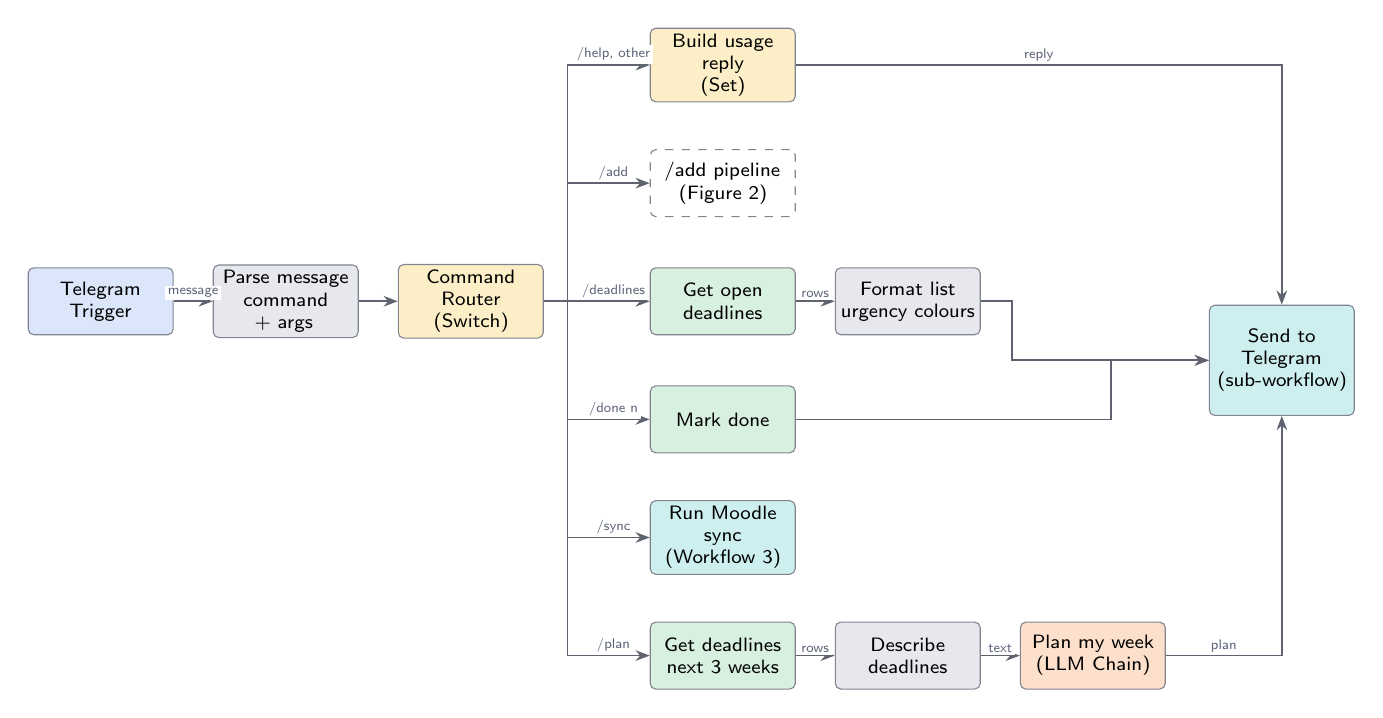
\begin{tikzpicture}
  \node[trig]  (tg)     at (0,0)      {Telegram Trigger};
  \node[code]  (parse)  at (2.35,0)   {Parse message\\ command + args};
  \node[logic] (router) at (4.7,0)    {Command Router\\ (Switch)};

  \node[logic] (help)   at (7.9,3.0)  {Build usage reply\\ (Set)};
  \node[ref]   (add)    at (7.9,1.5)  {/add pipeline\\ (Figure 2)};
  \node[db]    (list)   at (7.9,0)    {Get open\\ deadlines};
  \node[db]    (done)   at (7.9,-1.5) {Mark done};
  \node[sub]   (sync)   at (7.9,-3.0) {Run Moodle sync\\ (Workflow 3)};
  \node[db]    (pq)     at (7.9,-4.5) {Get deadlines\\ next 3 weeks};

  \node[code]  (fmt)    at (10.25,0)  {Format list\\ urgency colours};
  \node[code]  (desc)   at (10.25,-4.5) {Describe\\ deadlines};
  \node[ai]    (plan)   at (12.6,-4.5) {Plan my week\\ (LLM Chain)};

  \node[sub, minimum height=14mm] (send) at (15.0,-0.75) {Send to\\ Telegram\\ (sub-workflow)};

  \draw[arr] (tg) -- node[lbl,above]{message} (parse);
  \draw[arr] (parse) -- (router);
  \foreach \nd/\lb in {help/{/help, other}, add/{/add}, list/{/deadlines}, done/{/done n}, sync/{/sync}, pq/{/plan}}
    \draw[arr] (router.east) -- ++(0.3,0) |- node[lbl,pos=0.78,above]{\lb} (\nd.west);
  \draw[arr] (list) -- node[lbl,above]{rows} (fmt);
  \draw[arr] (pq) -- node[lbl,above]{rows} (desc);
  \draw[arr] (desc) -- node[lbl,above]{text} (plan);
  \draw[arr] (help.east) -| node[lbl,pos=0.25,above]{reply} (send.north);
  \draw[arr] (fmt.east) -- ++(0.4,0) |- (send.west);
  \draw[arr] (done.east) -- ++(4.0,0) |- (send.west);
  \draw[arr] (plan.east) -| node[lbl,pos=0.25,above]{plan} (send.south);
\end{tikzpicture}
\end{center}

{\footnotesize\color{muted}Both AI nodes (\emph{Extract deadline} and \emph{Plan my week}) also have an error output that replies `The AI is busy, try again'' (drawn in Figure 2 only).}

% ---------- Figure 2: /add ----------
\subsection{The /add pipeline (inside Main)}

\begin{center}
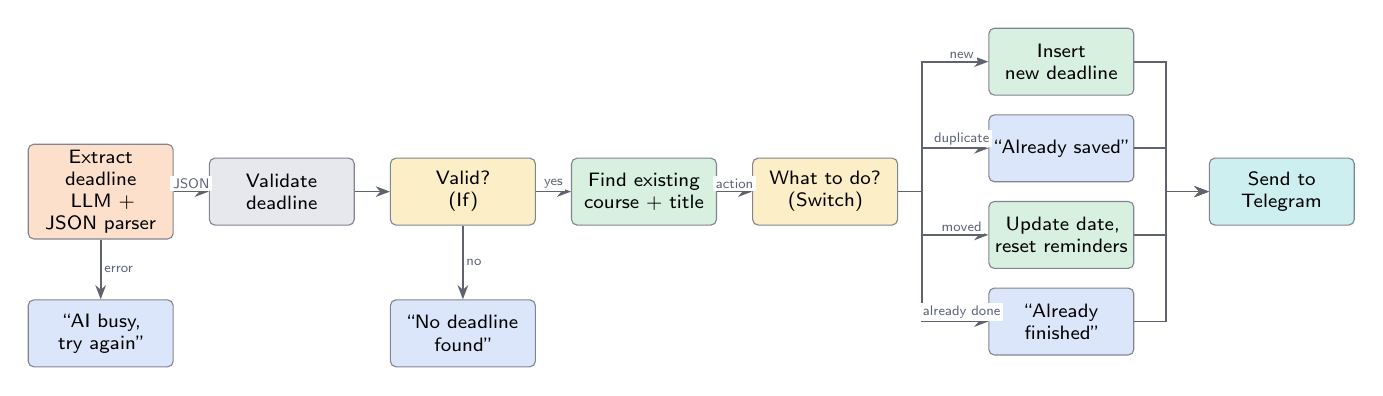
\begin{tikzpicture}
  \node[ai]    (ext)   at (0,0)      {Extract deadline\\ LLM + JSON parser};
  \node[code]  (val)   at (2.3,0)   {Validate\\ deadline};
  \node[logic] (ok)    at (4.6,0)    {Valid?\\ (If)};
  \node[db]    (find)  at (6.9,0)   {Find existing\\ course + title};
  \node[logic] (sw)    at (9.2,0)    {What to do?\\ (Switch)};

  \node[db]    (ins)   at (12.2,1.65)  {Insert\\ new deadline};
  \node[trig]  (dup)   at (12.2,0.55)  {``Already saved''};
  \node[db]    (mov)   at (12.2,-0.55) {Update date,\\ reset reminders};
  \node[trig]  (fin)   at (12.2,-1.65) {``Already\\ finished''};

  \node[trig]  (busy)  at (0,-1.8)   {``AI busy,\\ try again''};
  \node[trig]  (no)    at (4.6,-1.8) {``No deadline\\ found''};
  \node[sub]   (send)  at (15.0,0)   {Send to\\ Telegram};

  \draw[arr] (ext) -- node[lbl,above]{JSON} (val);
  \draw[arr] (val) -- (ok);
  \draw[arr] (ok) -- node[lbl,above]{yes} (find);
  \draw[arr] (ok) -- node[lbl,right]{no} (no);
  \draw[arr] (ext) -- node[lbl,right]{error} (busy);
  \draw[arr] (find) -- node[lbl,above]{action} (sw);
  \foreach \nd/\lb in {ins/new, dup/duplicate, mov/moved, fin/already done}
    \draw[arr] (sw.east) -- ++(0.3,0) |- node[lbl,pos=0.8,above]{\lb} (\nd.west);
  \foreach \nd in {ins, dup, mov, fin}
    \draw[arr] (\nd.east) -- ++(0.4,0) |- (send.west);
\end{tikzpicture}
\end{center}
\vspace{-4pt}
{\footnotesize\color{muted}The AI must answer in a fixed JSON shape (found, course, title, due, weight). The Code node
checks that the date really exists before anything is saved, because the AI's output is never trusted as it is.
``No deadline found'' and ``AI busy'' also go through Send to Telegram (arrows not drawn).}

% ---------- Figure 3: Reminders + Moodle sync ----------
\subsection{Workflows 2 and 3: morning reminders and Moodle sync}

\begin{center}
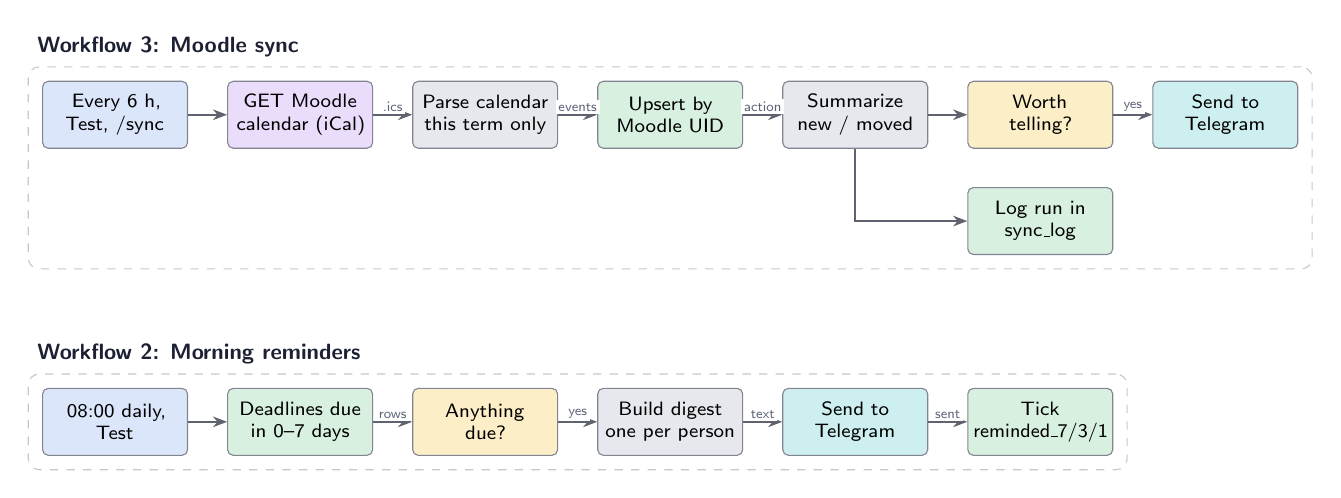
\begin{tikzpicture}
  % Moodle sync
  \node[trig]  (s1)  at (0,0)      {Every 6 h,\\ Test, /sync};
  \node[api]   (ics) at (2.35,0)   {GET Moodle\\ calendar (iCal)};
  \node[code]  (pc)  at (4.7,0)    {Parse calendar\\ this term only};
  \node[db]    (up)  at (7.05,0)   {Upsert by\\ Moodle UID};
  \node[code]  (sm)  at (9.4,0)    {Summarize\\ new / moved};
  \node[logic] (wt)  at (11.75,0)  {Worth\\ telling?};
  \node[sub]   (s2)  at (14.1,0)   {Send to\\ Telegram};
  \node[db]    (lg)  at (11.75,-1.35) {Log run in\\ sync\_log};
  \draw[arr] (s1) -- (ics);
  \draw[arr] (ics) -- node[lbl,above]{.ics} (pc);
  \draw[arr] (pc) -- node[lbl,above]{events} (up);
  \draw[arr] (up) -- node[lbl,above]{action} (sm);
  \draw[arr] (sm) -- (wt);
  \draw[arr] (wt) -- node[lbl,above]{yes} (s2);
  \draw[arr] (sm.south) |- (lg.west);
  \begin{scope}[on background layer]
    \node[frame, fit=(s1)(ics)(pc)(up)(sm)(wt)(s2)(lg)] (F3) {};
  \end{scope}
  \node[ftitle] at (F3.north west) {Workflow 3: Moodle sync};

  % Reminders
  \node[trig]  (r1)  at (0,-3.9)     {08:00 daily,\\ Test};
  \node[db]    (rq)  at (2.35,-3.9)  {Deadlines due\\ in 0--7 days};
  \node[logic] (ad)  at (4.7,-3.9)   {Anything\\ due?};
  \node[code]  (bd)  at (7.05,-3.9)  {Build digest\\ one per person};
  \node[sub]   (s3)  at (9.4,-3.9)   {Send to\\ Telegram};
  \node[db]    (mk)  at (11.75,-3.9) {Tick\\ reminded\_7/3/1};
  \draw[arr] (r1) -- (rq);
  \draw[arr] (rq) -- node[lbl,above]{rows} (ad);
  \draw[arr] (ad) -- node[lbl,above]{yes} (bd);
  \draw[arr] (bd) -- node[lbl,above]{text} (s3);
  \draw[arr] (s3) -- node[lbl,above]{sent} (mk);
  \begin{scope}[on background layer]
    \node[frame, fit=(r1)(rq)(ad)(bd)(s3)(mk)] (F2) {};
  \end{scope}
  \node[ftitle] at (F2.north west) {Workflow 2: Morning reminders};
\end{tikzpicture}
\end{center}

% ---------- Figure 4: sub-workflow + errors ----------
\subsection{Workflows 4 and 5: Send to Telegram and error handling}

\begin{center}
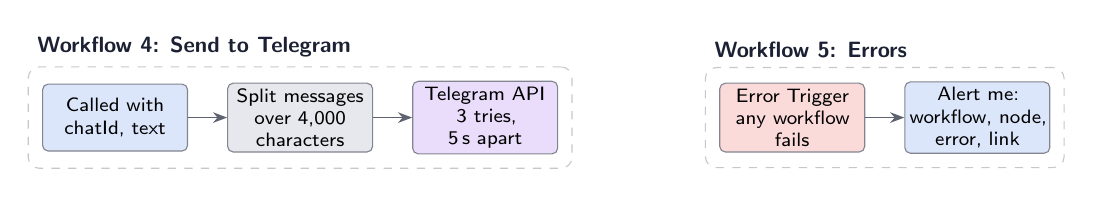
\begin{tikzpicture}
  \node[trig] (c1) at (0,0)     {Called with\\ chatId, text};
  \node[code] (sp) at (2.35,0)  {Split messages\\ over 4,000\\ characters};
  \node[api]  (tl) at (4.7,0)   {Telegram API\\ 3 tries,\\ 5\,s apart};
  \draw[arr] (c1) -- (sp);
  \draw[arr] (sp) -- (tl);
  \begin{scope}[on background layer]
    \node[frame, fit=(c1)(sp)(tl)] (F4) {};
  \end{scope}
  \node[ftitle] at (F4.north west) {Workflow 4: Send to Telegram};

  \node[err]  (et) at (8.6,0)   {Error Trigger\\ any workflow\\ fails};
  \node[trig] (al) at (10.95,0) {Alert me: workflow, node, error, link};
  \draw[arr] (et) -- (al);
  \begin{scope}[on background layer]
    \node[frame, fit=(et)(al)] (F5) {};
  \end{scope}
  \node[ftitle] at (F5.north west) {Workflow 5: Errors};
\end{tikzpicture}
\end{center}

\textbf{Database.} One Supabase (Postgres) table \cmd{deadlines}: course, title, due date, grade weight, status
(open or done), source (manual or moodle), the Moodle event ID (unique), and three flags \cmd{reminded\_7},
\cmd{reminded\_3} and \cmd{reminded\_1}. A second table \cmd{sync\_log} records each Moodle sync. Dates are stored in UTC
and converted to Paris time in the SQL, so the Python code never deals with time zones.

% ================= 4. Design choices =================
\section{Design choices}

\begin{itemize}
  \item \textbf{One job per workflow.} Receiving messages, reminders, syncing and error handling run on different
  triggers and fail independently. A broken Moodle feed cannot stop the bot from answering.
  \item \textbf{One sender for every message.} All replies go through the \emph{Send to Telegram} sub-workflow, which
  splits messages above Telegram's 4,096-character limit and retries. The other workflows only say ``send this text to
  this chat''. Only the error alert calls Telegram directly, so it still works if the sub-workflow itself is broken.
  \item \textbf{Never trust the AI blindly.} The AI is used for language (reading ``next monday'', writing a plan), never
  for storage decisions. Its output must match a JSON schema, then a Code node checks the date exists.
  \item \textbf{Idempotent sync and reminders.} The sync matches events on Moodle's unique ID, so running it twice
  changes nothing. Reminder flags are only ticked after Telegram confirms the message, so a failed send is retried the
  next day instead of being lost.
  \item \textbf{Ask the database to do the date maths.} Days left, Paris time and readable dates come from SQL, which
  keeps the Code nodes short and readable.
\end{itemize}

% ================= 5. Error handling =================
\section{Error handling and retries}

\begin{itemize}
  \item \textbf{Retry on fail} (3 tries) on both AI nodes, the Moodle download, the Telegram sender, and the database
  writes of the Moodle sync and the reminders.
  \item \textbf{AI failures:} free models are often rate-limited. If the retries still fail, the AI node's error output
  sends the user ``The AI is busy, try again in a minute'' instead of leaving them without an answer.
  \item \textbf{Bad input:} unknown commands get the usage message, typos get ``Did you mean \ldots?'', and messages
  without a date are refused before reaching the database.
  \item \textbf{Error workflow:} any other failure sends me a Telegram alert with the workflow, the failing node, the
  error message and a link to the execution. It proved useful for real: on 22 October at 08:00 the reminder digest failed (a chat ID read as text instead of a number). The alert pointed straight to the failing node and I fixed it the same morning. Because reminder flags are only ticked after a successful send, no reminder was lost.
\end{itemize}

% ================= 6. Requirements =================
\section{Minimum technical requirements}

\renewcommand{\arraystretch}{1.2}
\begin{tabularx}{\linewidth}{@{}>{\raggedright\arraybackslash}p{3.4cm} X@{}}
\toprule
\textbf{Requirement} & \textbf{Where it is in the project} \\
\midrule
If or Set node & If: \emph{Valid?}, \emph{Anything due?}, \emph{Worth telling?}. Set: \emph{Build usage reply}. \\
Code node & Python: Parse message, Validate deadline, Format list, Describe deadlines, Build digest, Parse calendar,
Summarize sync, Split long message. \\
Router or If/Switch & \emph{Command Router} (7 routes) and \emph{What to do?} (new / duplicate / moved / already done). \\
API connection & HTTP Request to the Moodle iCal export; OpenRouter API; Telegram Bot API; Supabase. \\
Message trigger & Telegram Trigger. \\
Database & Supabase (Postgres): \cmd{deadlines} and \cmd{sync\_log}. \\
AI node & Two LLM Chains: \emph{Extract deadline} (structured JSON output) and \emph{Plan my week}. \\
Sub-workflow & \emph{Send to Telegram}, called by Main, Reminders and Moodle Sync; \emph{Moodle sync}, called by \cmd{/sync}. \\
Error handling and retries & Retry on fail on the AI, HTTP and Telegram calls and the key database writes; error output on both AI nodes; Error Workflow. \\
\bottomrule
\end{tabularx}

% ================= 7. Level and changes =================
\section{Level reached, and what changed since the proposal}

\textbf{Level 3.} The system keeps state between runs (reminder flags, Moodle event IDs), detects duplicates and
date changes, uses sub-workflows and an error workflow, and retries the calls most likely to fail.

\begin{itemize}
  \item \textbf{AI provider:} OpenRouter free models instead of Groq, as in the course lab.
  \item \textbf{Sub-workflow:} instead of \emph{Parse \& Save}, the shared sub-workflow is \emph{Send to Telegram}. It
  is used by every workflow that replies to the user, which made it the more useful one to extract. Duplicate detection stayed in Main.
  \item \textbf{Moodle sync:} one SQL ``upsert'' returns new, moved or unchanged for each event, instead of a separate
  Switch. A summary message is sent only when something changed.
  \item \textbf{\cmd{/plan}:} built as an LLM Chain that receives the deadlines as text, rather than an AI Agent with a
  database tool. It is simpler and the data the AI sees is always exactly what the database holds.
  \item \textbf{Found while building:} the Moodle calendar only contains deadlines created as Moodle activities. Many
  deadlines are only announced in class or in course documents, so \cmd{/add} remains essential.
\end{itemize}

% ================= 8. WhatsApp =================
\section{What would change on WhatsApp}

The design would stay the same; only the two ends change. The Telegram Trigger would become the WhatsApp Trigger, fed
by a Meta Cloud API webhook that has to be verified, and \emph{Send to Telegram} would become \emph{Send to WhatsApp}
using the WhatsApp Business Cloud node. Because every message already goes through that one sub-workflow, only one
workflow would change. Two WhatsApp rules affect this project: the bot can only message registered numbers, and outside
24 hours after the user's last message it can only send pre-approved templates. The 08:00 reminder would therefore have
to be an approved template, while replies to commands would work as they do now.

% ================= 9. Limits =================
\section{Limits and possible improvements}

\begin{itemize}
  \item Duplicate detection matches the exact course and title, so ``Final report'' and ``Final project report'' count
  as two deadlines. Fuzzy matching would fix this.
  \item A deadline added by hand can also arrive later from Moodle, giving two rows.
  \item Deadlines that are not on Moodle need \cmd{/add}. A next step would be to forward a document to the bot and let the
  AI extract every deadline in it.
  \item Free AI models are slow and rate-limited. A paid model would make \cmd{/add} and \cmd{/plan} faster and more
  reliable.
\end{itemize}

\textbf{Use of AI.} I used an AI assistant to help design the workflows and to draft and review the Code nodes and SQL
queries. I built, tested and adjusted every node myself in n8n, and I can explain each of them.

\end{document}
